\documentclass{article}


% if you need to pass options to natbib, use, e.g.:
\PassOptionsToPackage{numbers}{natbib}
% before loading neurips_2023


% ready for submission
% \usepackage{neurips_2023}


% to compile a preprint version, e.g., for submission to arXiv, add add the
% [preprint] option:
%     \usepackage[preprint]{neurips_2023}


% to compile a camera-ready version, add the [final] option, e.g.:
    \usepackage[final]{neurips_2023}


% to avoid loading the natbib package, add option nonatbib:
%    \usepackage[nonatbib]{neurips_2023}


\usepackage[utf8]{inputenc} % allow utf-8 input
\usepackage[T1]{fontenc}    % use 8-bit T1 fonts
\usepackage{hyperref}       % hyperlinks
\usepackage{url}            % simple URL typesetting
\usepackage{booktabs}       % professional-quality tables
\usepackage{amsfonts}       % blackboard math symbols
\usepackage{nicefrac}       % compact symbols for 1/2, etc.
\usepackage{microtype}      % microtypography
\usepackage{xcolor}         % colors

\usepackage{bm}
\usepackage[noline,ruled]{algorithm2e}
\usepackage{cleveref}
\usepackage{graphicx}
\usepackage{caption}
\usepackage{subcaption}

\title{C3: Federated Learning with Iterative Moving Averaging In-Depth an Experimental Perspective}


% The \author macro works with any number of authors. There are two commands
% used to separate the names and addresses of multiple authors: \And and \AND.
%
% Using \And between authors leaves it to LaTeX to determine where to break the
% lines. Using \AND forces a line break at that point. So, if LaTeX puts 3 of 4
% authors names on the first line, and the last on the second line, try using
% \AND instead of \And before the third author name.


\author{%
  Jedidiah Koh \\
  Department of Computer Science\\
  University of Cambridge\\
  United Kingdom \\
  \texttt{jk810@cam.ac.uk} \\
  % examples of more authors
  % \And
  % Coauthor \\
  % Affiliation \\
  % Address \\
  % \texttt{email} \\
  % \AND
  % Coauthor \\
  % Affiliation \\
  % Address \\
  % \texttt{email} \\
  % \And
  % Coauthor \\http://jmlr.csail.mit.edu/papers/volume3/blei03a/blei03a.pdf
  % Affiliation \\
  % Address \\
  % \texttt{email} \\
  % \And
  % Coauthor \\
  % Affiliation \\
  % Address \\
  % \texttt{email} \\
}


\newcommand*{\fedavg}{\textsc{FedAvg}}

\begin{document}


\maketitle


\begin{abstract}
  Federated Learning has been shown to be able to yield good results using model averaging even when trained on heterogeneous clients. However, the global model still deviates from the expected minimum and this loss can be partly attributed to the non-overlapping data of clients. Iterative moving average has been used to mitigate this effects and has been shown to improve model accuracy. Here, I investigate the effects of heterogeneity on model training and how it affects both the global averaged model and individual clients in terms of the their output activations. I show that client label distribution is correlated with the change in the output activations of the model and that IMA mitigates the effects in the global model.
\end{abstract}

\section{Introduction}
Federated Learning (FL) is the training of neural networks in a distributed fashion across multiple clients with usually private datasets. Model averaging with \fedavg{} \cite{mcmahanCommunicationEfficientLearningDeep2017} has been shown to be surprisingly effective in achieving convergence even under conditions of data heterogeneity and non-convex loss functions. However, \citet{zhouUnderstandingImprovingModel2023} have shown that the performance of \fedavg{} on heterogeneous datasets is limited by the \emph{heterogeneity bias}, which is due to the non-overlapping nature of the data distributions across clients. They propose \emph{iterative moving averaging} (IMA) as a method to mitigate the heterogeneity bias and bring the model to the center of the loss basin.

In this project, I look at the effects of heterogeneous clients on the training of the federated model by analysing the activation outputs of the client and global models when iterative moving averaging is used. I also consider how the underlying distribution of the client dataset corresponds with the activation outputs of the local model trained on a client. In summary my contributions are:
\begin{itemize}
  \item Creating heterogeneous partitions of the CIFAR-10 dataset using Latent Dirichlet Allocation
  \item Performing FL training using \fedavg{} with IMA on the created partitions
  \item Showing that data label distribution correlates with changes to the activation outputs and that the model averaging strategy helps to mitigate this effect on the global model.
\end{itemize}

\section{Background}
\subsection{Federated Learning with \fedavg}
FL is a more restricted scenario of distributed learning. The distributed machines are no longer under the control of the central server, but are often private client machines across the internet. Datasets are also no longer centralised but are distributed across the clients, and furthermore, private to them. FL involves training a model across these clients without having to transfer the underlying dataset back to the central server, thus preserving privacy and also reducing communication costs.

\fedavg{} is a FL model averaging method that relies on clients doing $n$ number of epochs on their own data and then averaging the models that each client returns to the server \cite{mcmahanCommunicationEfficientLearningDeep2017}. This constitutes one server round, but the ability to increase $n$ allows for more training to be done with less communication overhead since the model parameters only have to be transmitted once per server round at the end of the $n$ epochs.

\subsection{Data Heterogeneity and Latent Dirichlet Allocation}
One of the main problems that plagues FL is data heterogeneity. Unlike centralised training that has a view of all the data, the siloed nature of FL means that each client is a distribution of data on its own. Data heterogeneity happens when the data distributions across clients are non-identical, and breaks many assumptions that can be made about training. The stochastic nature of FL when picking clients at random means that at each round of training the data distribution can vary widely. Without the assumption that all clients have Independant and Identical Distributions (IID), we cannot assert that the stochastic gradient at each round is an unbiased estimate of the full gradient \cite{zhaoFederatedLearningNonIID2018} and thus there is a limit to how low we can bound the loss \cite{karimireddySCAFFOLDStochasticControlled2021}. \citet{zhouUnderstandingImprovingModel2023} model this irremovable error with \emph{Heterogeneity Bias} and show how it can degrade model training due to catastrophic forgetting.

For training purposes, a centralized dataset can be parittioned in a heterogeneous way using Latent Dirichlet Allocation (LDA) \cite{bleiLatentDirichletAllocation2003a}. Given a bag of $K$ words, we can create topics, which are multinomial distributions over the words. LDA then involves selecting a topic using a dirichlet distribution, which generates a tuple $(p_1,\ldots,p_K)$ such that $\sum p_i=1$, effectively generating the probabilities of a multinomial distribution of the $K$ words. The dirichlet distribution is parameterised by a \emph{concentration} parameter $\bm{\alpha} \in \mathbb{R}^{K}, \alpha_i > 0$ that affects how skewed the resulting output is \cite{frigyikIntroductionDirichletDistribution2010}. If we treat all words equally and set $\alpha_i=\alpha\forall i\in \{1,2,\ldots K\}$  for some constant $\alpha$, then the higher $\alpha$ is, the more likely we are to get an output tuple of $p_i$ that are approximately equal. Conversely, the lower $\alpha$ is, the more likely we are to get a skewed distribution over the words (e.g. $p_k\approx 1$ and $p_i\approx 0$ for $i\neq k$). Given any dataset, we can treat the features or labels as words, and partitions as topics to create synthetic heterogeneous datasets with feature distribution skew or label distribution skew.

Nevertheless, data heterogeneity happens naturally in most FL applications because of the way data is generated. Edge devices are often different low-end machines like mobile phones that are each usually only used by a single person. For example, in a Natural Language Processing (NLP) setting, each person has their own unique preference for words and phrases \cite{fallahPersonalizedFederatedLearning2020} that they use and a keyboard app on the users' mobile phones will have different word and ngram distributions across different phones. When training models on these heterogeneous clients, the models shift towards the local minima of the clients, which are often different from each other and also different from the global minimum. This common situation is know as \emph{client drift} and provides great motivation for studying FL methods that can handle heterogeneous conditions.

\subsection{Other FL methods}
Since \fedavg{}, other model averaging methods have been developed that improve FL robustness under real world conditions. For example, \textsc{FedProx} \cite{liFederatedOptimizationHeterogeneous2020} limits client drift by bounding gradient updates from client training at the expense of convergence rates. \textsc{FedOpt} \cite{reddiAdaptiveFederatedOptimization2021} incorporates well-known adaptive optimisers like \textsc{Adagrad}, \textsc{Adam} and \textsc{Yogi} \cite{duchiAdaptiveSubgradientMethods2011,kingmaAdamMethodStochastic2017,zaheerAdaptiveMethodsNonconvex2018}.  \textsc{FedMed} deals with the security issue of Byzantine-faulty machines participating in training by using coordinate wise-median to avoid getting skewed by the erroneous machine's training results.

\subsection{Iterative Moving Averaging}
In this project, I investigate Iterative Moving Averaging (IMA), where a time window over the recent FL rounds is maintained and the global model is the average of the trained models in this window \cite{zhouUnderstandingImprovingModel2023}. As the authors explain, the stochastic nature of model averaging causes the client drift at each round to shift the model away from the global minimum and towards the clients' local minima.
As found by the auhtors, client models tend to reside on the edge of the loss basin instead of at the global minimum in the center, but their averaged model falls nearer the center of the basin and closer to the minimum. Training on a subset of the clients thus shifts the model towards the edges and in addition to shifting it away from the minimum, also shifts it away from client mimima on the opposite side of the basin. This possibly undoes work from previous rounds when training on other clients and is an example of catastrophic forgetting. In this case, the catastrophic forgetting happens within the task and examples that are learnt from later clients causes the model to forget examples learnt from earlier clients. The heterogeneous nature of the data means that the new information gained and the old information forgotten come from different distributions of the global dataset, which is what degrades performance. IMA mitigates this by averaging over the sliding window of past rounds, and this explicit retention of information from past rounds reduces the ``forgetfulness'' of the model.


\section{Methods}
I follow the IMA algorithm introduced by \citet{zhouUnderstandingImprovingModel2023} that I reproduce below in \cref{alg:IMA}. The server keeps a time window of the model parameters obtained using normal Federated Model Averaging (FMA) for the last $P$ rounds. This model can be obtained with any model averaging algorithm of one's choice. I use \fedavg{} in this project. Before round $t_s$, we only perform FMA and do not use IMA, which reduces the noise from models from the intial stages of training. From round $t\geq t_s$ onwards, the model $\mathbf{w}^{(t)}$ is stored and instead of using it for the next round of training, we use the IMA model given by
\[\mathbf{w}^{(t)}_{\mathrm{IMA}} = \frac{1}{P}\sum_{i=0}^{P-1}\mathbf{w}^{(t-i)}\]

Additionally, the authors investigated how client models tend to reside at the wall of the loss basin instead of at the center. To avoid the model leaving the loss basin during the IMA phase, a stronger learning rate decay is adopted.

\begin{algorithm}
  \caption{FL with IMA}\label{alg:IMA}
  \SetKwInOut{Input}{Input}
  \SetKwFor{OnClient}{on client}{do}{end on client}
  \Input{model $\mathbf{w}$, total client number $K$, IMA's start round $t_s$, IMA's window size $P$}
  \For{each round t=1,$\cdots$, $R$}{
  Server samples clients $S\subseteq [K]$\;
  \eIf{$\geq t_s$}{
  Server sends $\mathbf{w}^{(t-1)}_{\mathrm{IMA}}$ to all clients $i\in S$
  }{Server sends $\mathbf{w}^{(t-1)}$ to all clients $i\in S$}
  \OnClient{$i \in S$ \KwSty{in parallel}}{
  \eIf{$t\geq t_s$}{
  Initialize the local model $\mathbf{w}_i\leftarrow\mathbf{w}^{(t-1)}_{\mathrm{IMA}}$\;
  Local training with mild exploration and get $\mathbf{w}_i^{(t)}$\;
  }{
  Initialize the local model $\mathbf{w}_i\leftarrow\mathbf{w}^{(t-1)}$\;
  Local training and get $\mathbf{w}_i^{(t)}$\;
  }
  Send $\mathbf{w}_i^{(t)}$ back to the server\;
  }
  Server perfroms FMA $\mathbf{w}_i^{(t)}\leftarrow \sum_{i\in S}(n_i/\sum_{i\in S}n_i)\mathbf{w}_i^{(t)}$\;
  \uIf{$t\geq t_s$}{
  Server performs IMA $\mathbf{w}^{(t)}_{\mathrm{IMA}}\leftarrow\frac{1}{P}\sum_{\tau=0}^{P-1}\mathbf{w}_i^{(t-\tau)}$\;
  }
  }
\end{algorithm}


\section{Experimental Setup and Methodology}
Given the effects of client drift on the training of the global model, I expect these effects to propagate into the activation patterns of the global model. Since a client that has a lot of data for label $x$ will push the activations for label $x$ upwards, we should expect to see a correlation between the label distributions on the client data and the activation outputs of the global model.

\subsection{Data Preparation}
I make use of the CIFAR-10 dataset \cite{krizhevskyLearningMultipleLayers2009} and apply appropriate normalisation transforms to normalise the pixel data to a mean of 0 and standard deviation of 1 \cite{ValueMeanStd2017}. I then synthetically heterogenise the dataset by paritioning it into 100 clients using the LDA code provided during the L361 labs \footnote{\tiny\url{https://github.com/camlsys/L361-Federated-Learning/blob/release/labs/common/lda_utils.py}}.

LDA is performed on the dataset with respect to the labels to create partitions with label distribution skew. A concentration value $\alpha$ is chosen and for each partition, a label distribution is generated from the dirchlet distribution parameterised by $\bm{\alpha}=(\alpha,\ldots,\alpha)\in\mathbb{R}^K$, where $K=10$ since there are 10 categories in our image dataset. This label distribution parameterises a multinomial distribution over the labels, which we then use to sample without replacement from the dataset. We repeat the label distribution generation and dataset sampling for each partition. Concentration values of $0.1, 1.0, 1000.0$ were used to generate the partitions. A visualisation of 5 paritions from each concentration value is shown in \cref{fig:label_freq_partial}. As can be seen from the bar plots, partitions generated by the concentration of 0.1 mainly consist of one to two labels, while partitions generated by the concentration of 1000.0 are generally even, and partitions generated with the concentration of 1.0 fall somewhere in between. The full data distribution across all clients can be found in \cref{full-data-dist}.

\begin{figure}
  \centering
  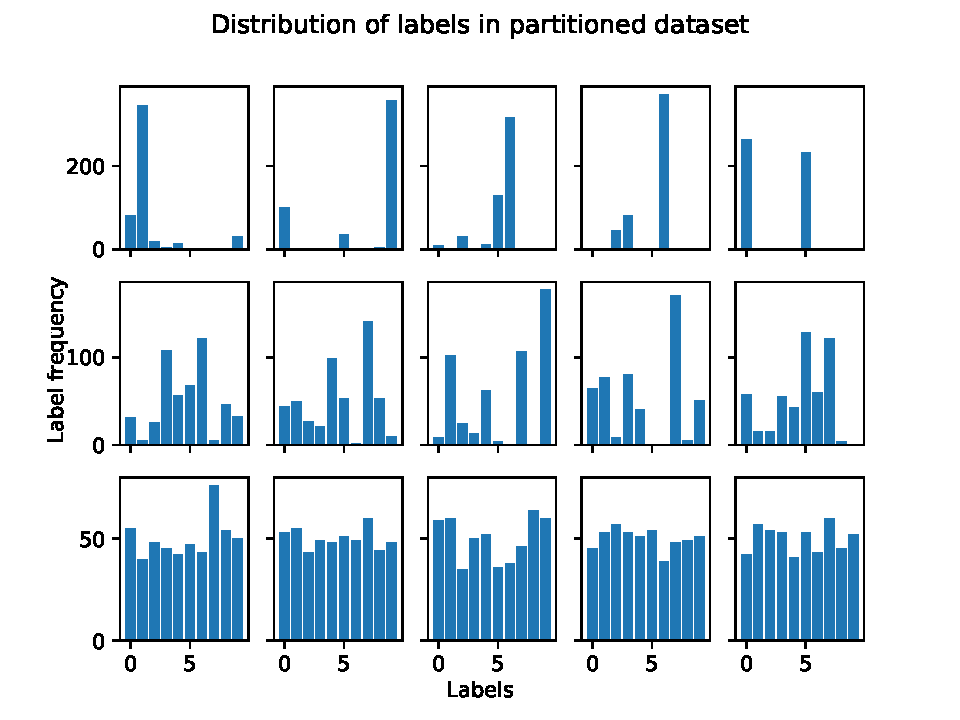
\includegraphics[width=0.7\textwidth]{images/label_dist_partial}
  \caption{Distribution of labels in 5 random partitions from each of the 3 concentrations of $0.1$ (top row), $1.0$ (middle) and $1000.0$ (bottom).}
  \label{fig:label_freq_partial}
\end{figure}

\subsection{Model}
Two models were tested, a 3-layer convolutional neural network (CNN) taken from the tensorflow tutorial \cite{ConvolutionalNeuralNetwork2024} and a 2-layer CNN (2CNN) used by \citet{zhouUnderstandingImprovingModel2023} that is based off \cite{mcmahanCommunicationEfficientLearningDeep2017}. The 2-layer CNN has three fully-connected layers after the convolutional layers, while the 3-layer CNN (3CNN) has two. Model parameters are shown in \cref{tbl:model_params}.

\begin{table}
  \centering
  \begin{tabular}{cc}
    \hline
    2CNN             & 3CNN            \\
    \hline
    conv(3,64,5)     & conv(3,32,3)    \\
    \multicolumn{2}{c}{maxpool(2x2)}   \\
    conv(64,64,5)    & conv(32,64,3)   \\
    linear(1600,384) & conv(64,64,3)   \\
    linear(384,128)  & linear(1024,64) \\
    linear(128,10)   & linear(64,10)
  \end{tabular}
  \caption{Model parameters used for training. The 3CNN model was chosen for further experiments.}
  \label{tbl:model_params}
\end{table}

\subsection{Training a starting model}
Both models were trained on the entire dataset for 40 epochs in a conventional setting without federated learning. Their performance on both a validation set and the centralised test set was monitored and is shown in \cref{fig:central_train}. Due to the lack of anything significant in the later half of training only the first 25 epochs are shown.

Both models showed similar performance on the test set and the only extra performance of the 2CNN comes from the training set, which is likely overfitting. Furthermore, the 2CNN takes longer to train than the 3CNN as shown in \cref{tbl:train_time}. I decided to focus my efforts on the 3CNN for the further experiments. Given that the accuracy starts to have large dips from round 10 onwards, I chose the model at round 5 to be the starting point of the subsequent experiments.

\begin{figure}
  \centering
  \begin{subfigure}[b]{0.45\textwidth}
    \centering
    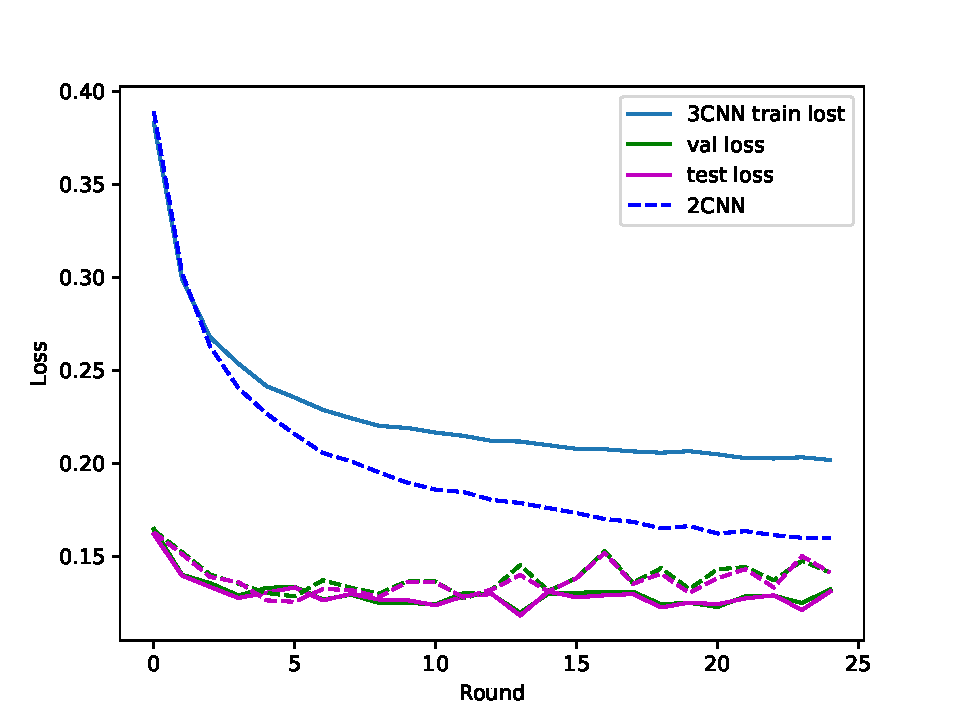
\includegraphics[width=0.7\textwidth]{images/initial_training}
    \caption{Loss values from centralised training.}
    \label{fig:central_train_loss}
  \end{subfigure}
  \hfill
  \begin{subfigure}[b]{0.45\textwidth}
    \centering
    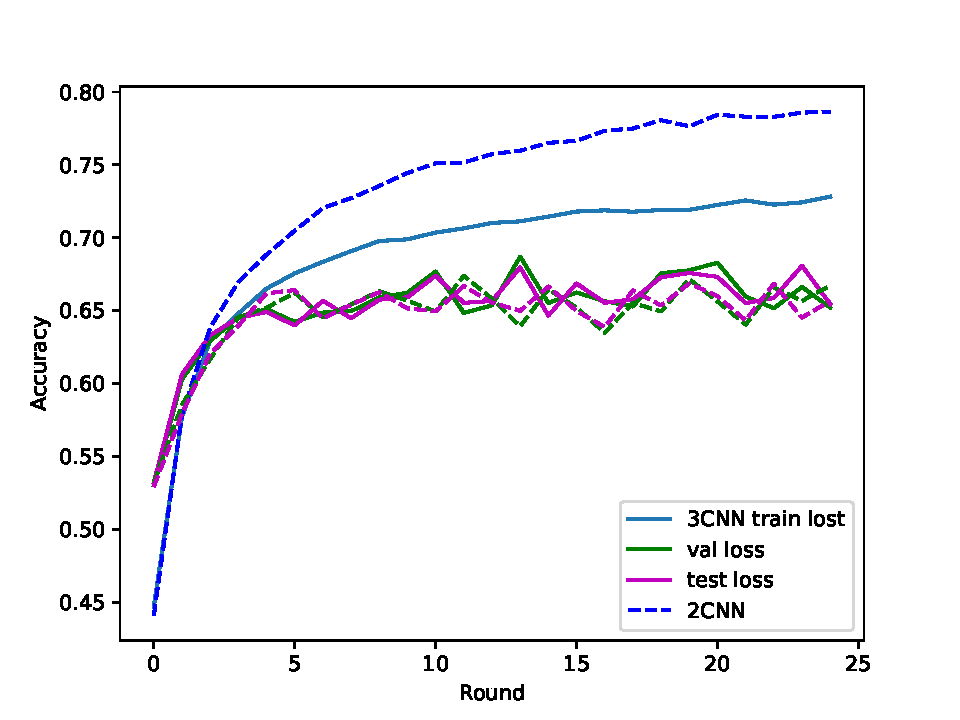
\includegraphics[width=0.7\textwidth]{images/initial_training_acc}
    \caption{Accuracy from centralised training.}
    \label{fig:central_train_acc}
  \end{subfigure}

  \caption{Metrics from centralised training. It can be seen that both the 3CNN and 2CNN models reach similar performance levels on the validation and test set, and the only improvement of the 2CNN model is on the training set, which is a likely sign of overfitting.}
  \label{fig:central_train}
\end{figure}

\begin{table}
  \centering
  \begin{tabular}{cc}
    \hline
    Model & Training time (s) \\
    \hline
    2CNN  & 4958              \\
    3CNN  & 3546
  \end{tabular}
  \caption{Training time of models over 40 epochs}
  \label{tbl:train_time}
\end{table}

\subsection{Federated Training and Analysis}
Using the starting point from the centralised training, I ran 400 rounds of federated learning on each of the partition sets using a strategy of \fedavg{} with IMA was used. The parameters used are shown in \cref{tbl:params}. I also ran the same training without IMA as a comparison. In addition to the usual accuracy and loss metrics, I recorded down the average activation output from 5 random tensors drawn from $\mathcal{U}(-1,1)$, the range is chosen as after normalisation of the CIFAR dataset its values are transformed into a distribution with mean 0 and standard deviation of 1. I also get the average activation output and confusion matrix when the model is run on the centralised test set. In addition to evaluating the global model that IMA returns, I also evaluate the same metrics on the individual clients that are used for training in each round and note the client cids used each round.

\begin{table}
  \centering
  \begin{tabular}{cc}
    \hline
    Parameters                      \\
    \hline
    $t_s$                    & 150  \\
    Start learning rate (LR) & 0.01 \\
    LR decay                 & 0.01 \\
    IMA LR decay             & 0.03 \\
    Batch size               & 50   \\
    \hline
  \end{tabular}
  \caption{Parameters used for training}
  \label{tbl:params}
\end{table}

FL training was done with the flower framework \footnote{\url{https://flower.ai/}}. In order to perform the individual client evaluation with the flower framework, I modified the strategy class to store the client parameters and client ids during the training phase of a round, and use them in the evaluation phase so as to evaluate the client models in addition to the global model.

The flower framework helps to ensure reproducibility by performing seeding of all random actions. A fixed seed value of 1337 was used throughout the experiments.

\section{Results and Discussion}
The loss and accuracy across the training rounds is shown in \cref{fig:training_loss_acc}. The difference in the distributions of the paritions can be immediately noticed from the large fluctatuations in training loss values for lower concentrations. The slight deviation between the experiments with and without IMA can be seen from round 150 onwards when IMA is used and the training with IMA demonstrates slightly more stability.

\begin{figure}
  \centering
  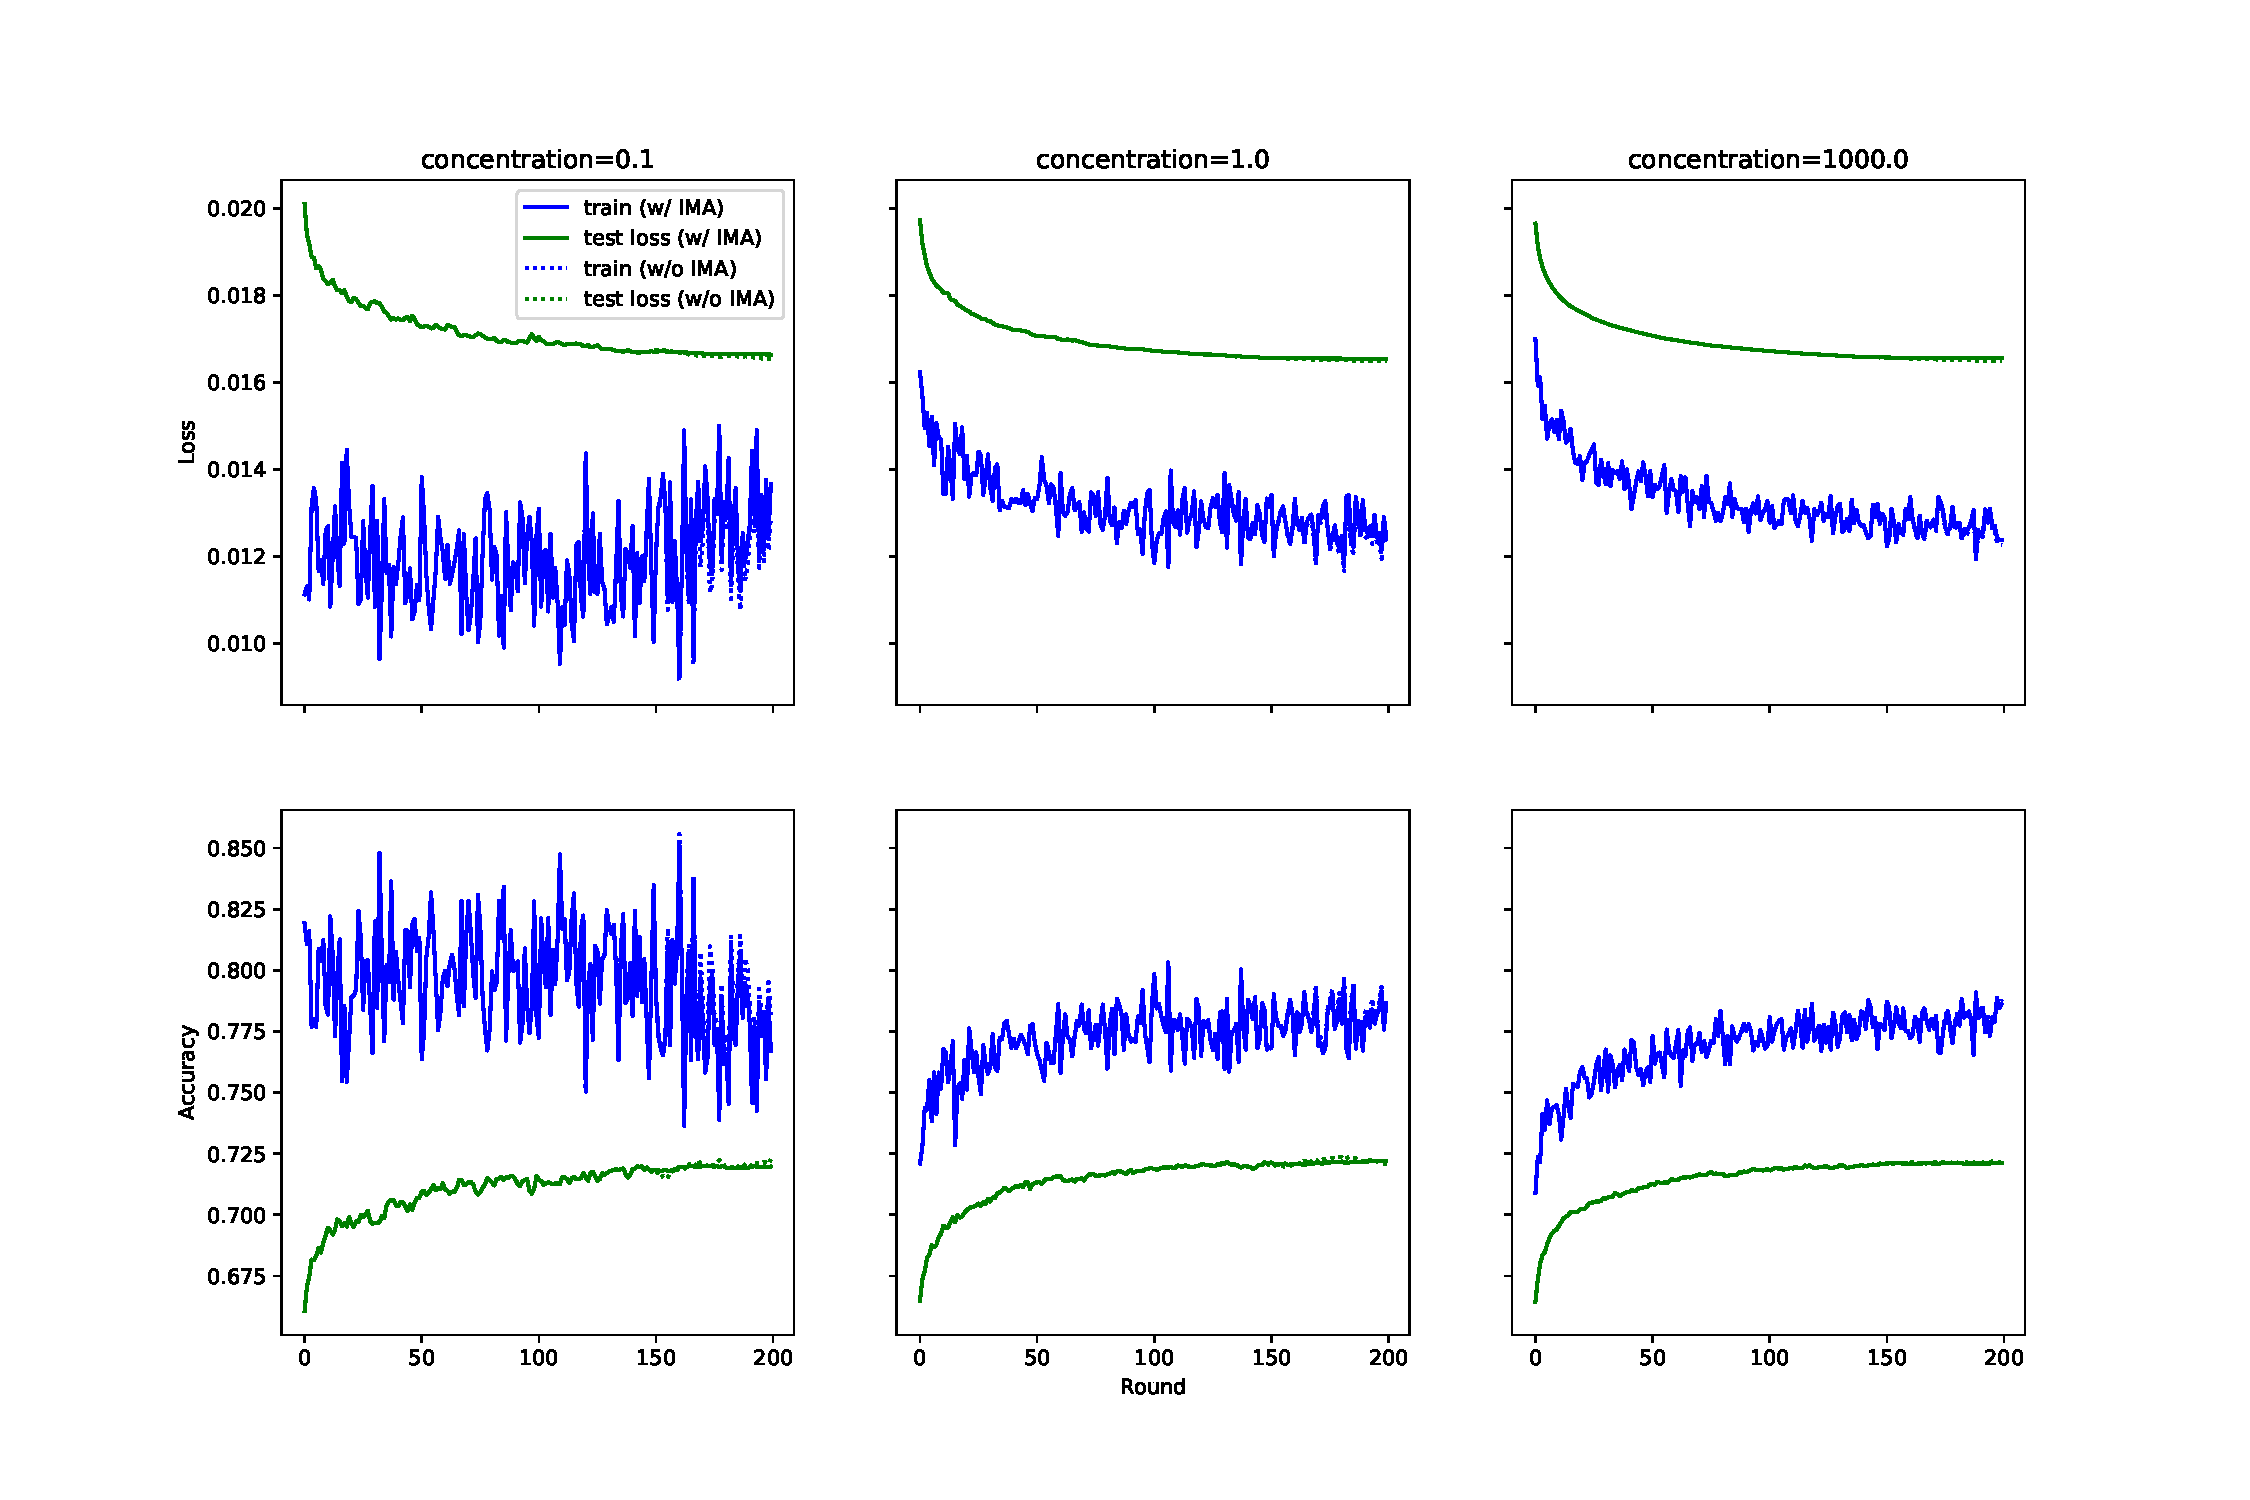
\includegraphics[width=0.9\textwidth]{images/training_hist.pdf}
  \caption{Loss and accuracy during training.}
  \label{fig:training_loss_acc}
\end{figure}

\subsection{Random Noise Activations}
When random noise is passed through the model across all rounds, we obtained the mean activation values for each label shown in \cref{fig:noise_activations}. There is no obvious difference between concentration values, and I suspected that given a more heterogeneous dataset, we could expect the activation outputs to have greater fluctuations. However, as can be seen from \cref{fig:fluct}, I do not have enough certainty to make such a conclusion. There is a slight decrease in the fluctuations as concentration increases, however they all fall within each others' error bars.

\begin{figure}
  \centering
  \begin{subfigure}[b]{0.32\textwidth}
    \centering
    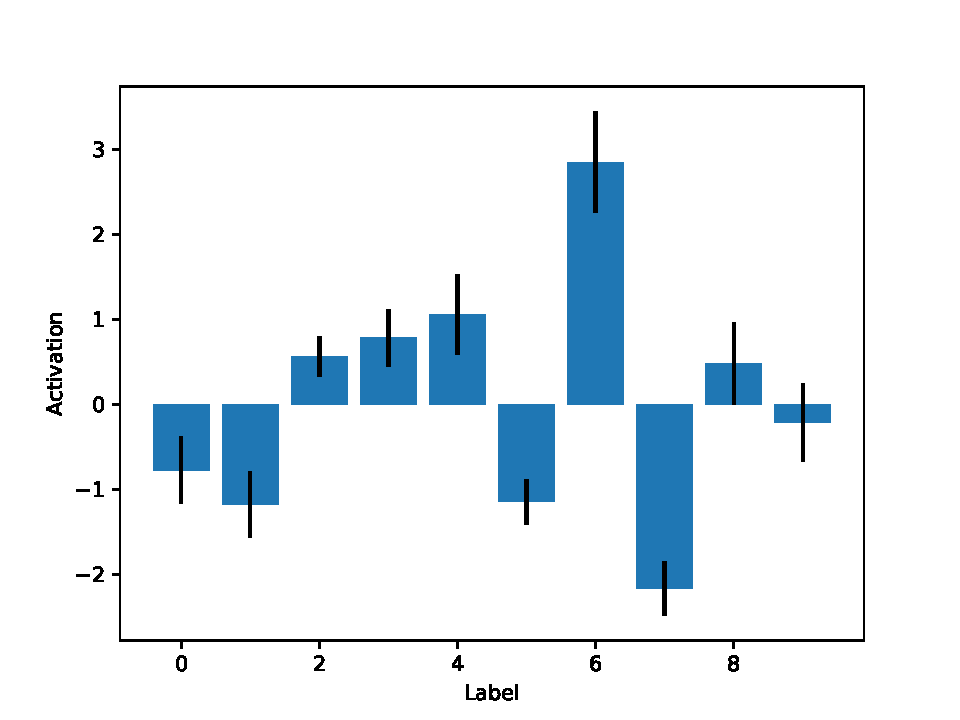
\includegraphics[width=\textwidth]{images/noise_activations_by_label_0.1.pdf}
    \caption{concentration of 0.1}
    \label{fig:noise_activations_0.1}
  \end{subfigure}
  \hfill
  \begin{subfigure}[b]{0.32\textwidth}
    \centering
    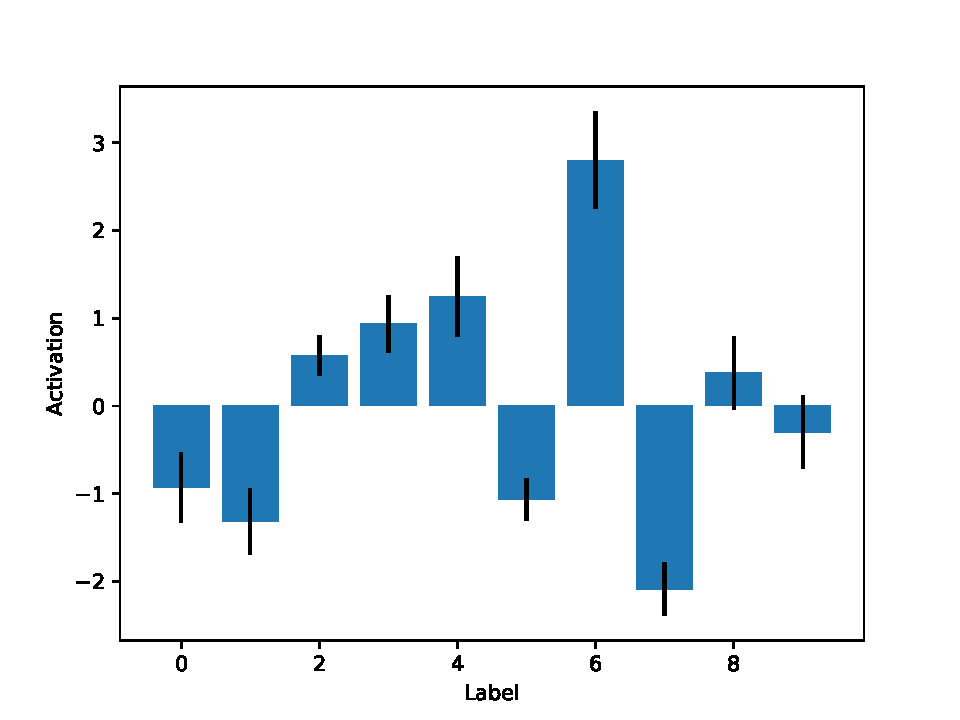
\includegraphics[width=\textwidth]{images/noise_activations_by_label_1.0.pdf}
    \caption{concentration of 1.0}
    \label{fig:noise_activations_1.0}
  \end{subfigure}
  \hfill
  \begin{subfigure}[b]{0.32\textwidth}
    \centering
    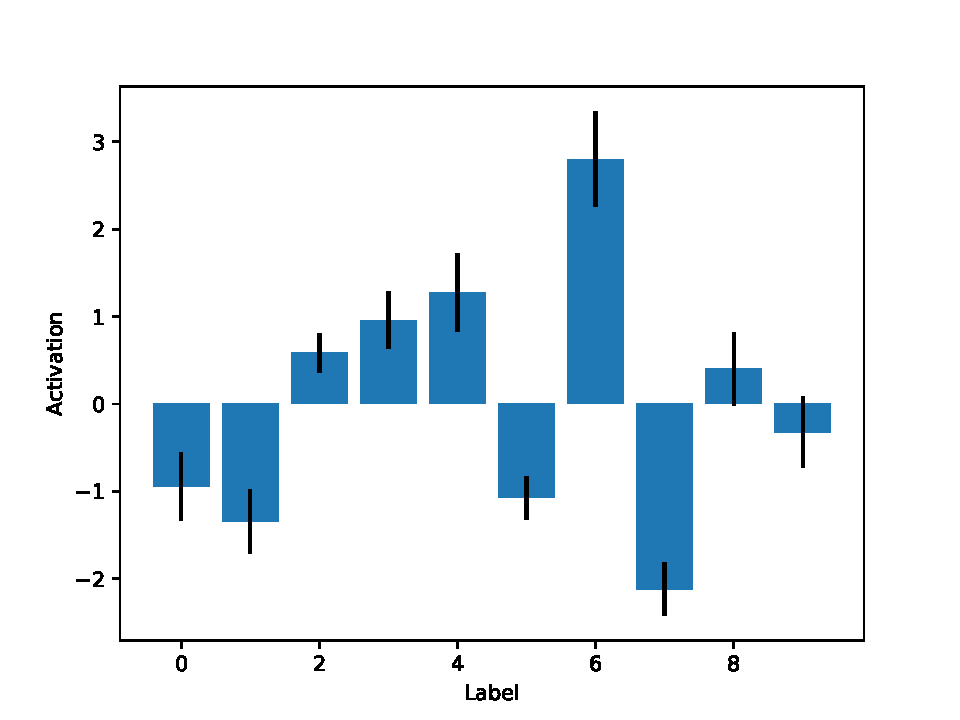
\includegraphics[width=\textwidth]{images/noise_activations_by_label_1000.0.pdf}
    \caption{concentration of 1000.0}
    \label{fig:noise_activations_1000.0}
  \end{subfigure}

  \caption{Model activations from random noise across all 200 rounds of training.}
  \label{fig:noise_activations}
\end{figure}

\begin{figure}
  \centering
  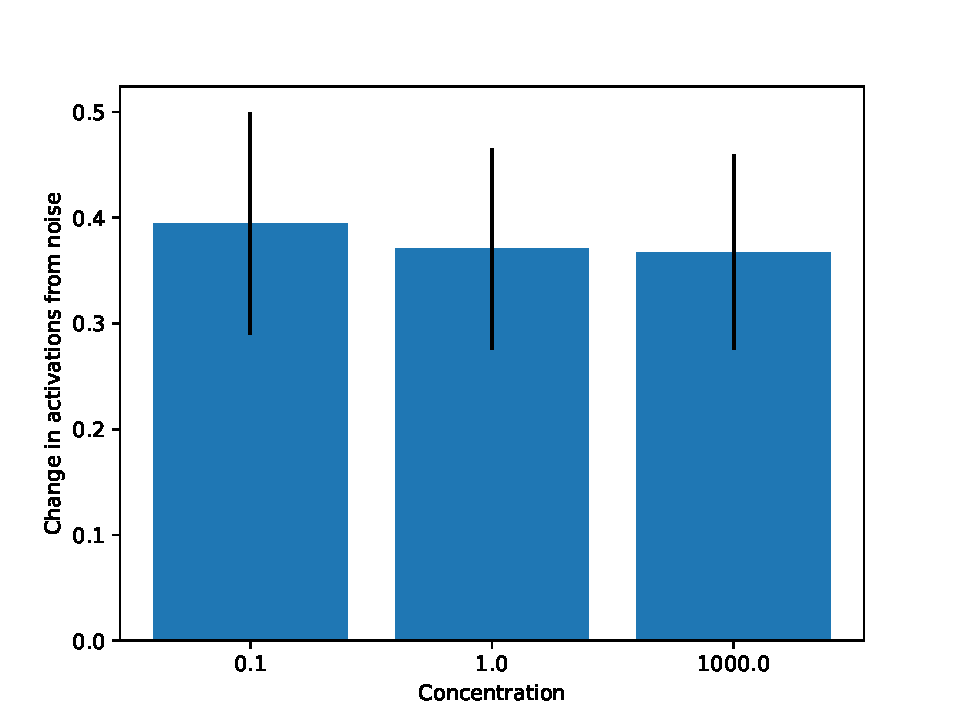
\includegraphics[width=0.6\textwidth]{images/noise_activation_change.pdf}
  \caption{Mean fluctuations of activation outputs. Fluctuations are calculated by taking the standard deviation of the activation outputs of a given label across all training rounds.}
  \label{fig:fluct}
\end{figure}

I also check the correlation between the activations and the client data distribution. As mentioned, if a client has more data from a specific label, we expect the activations for that label to increase as well. In order to make a fair comparison, I also compare the correlation between the activations and 3 sets of 10 randomly selected client datasets from the same concentration. However, as can be seen from \cref{fig:noise_client}, the data seems too noisy to draw any conclusions, although we can notice a drop in the correlation at the beginning of the training for a concentration of 0.1. This decrease could likely be attributed to the learning rate decay of the strategy.

\begin{figure}
  \centering
  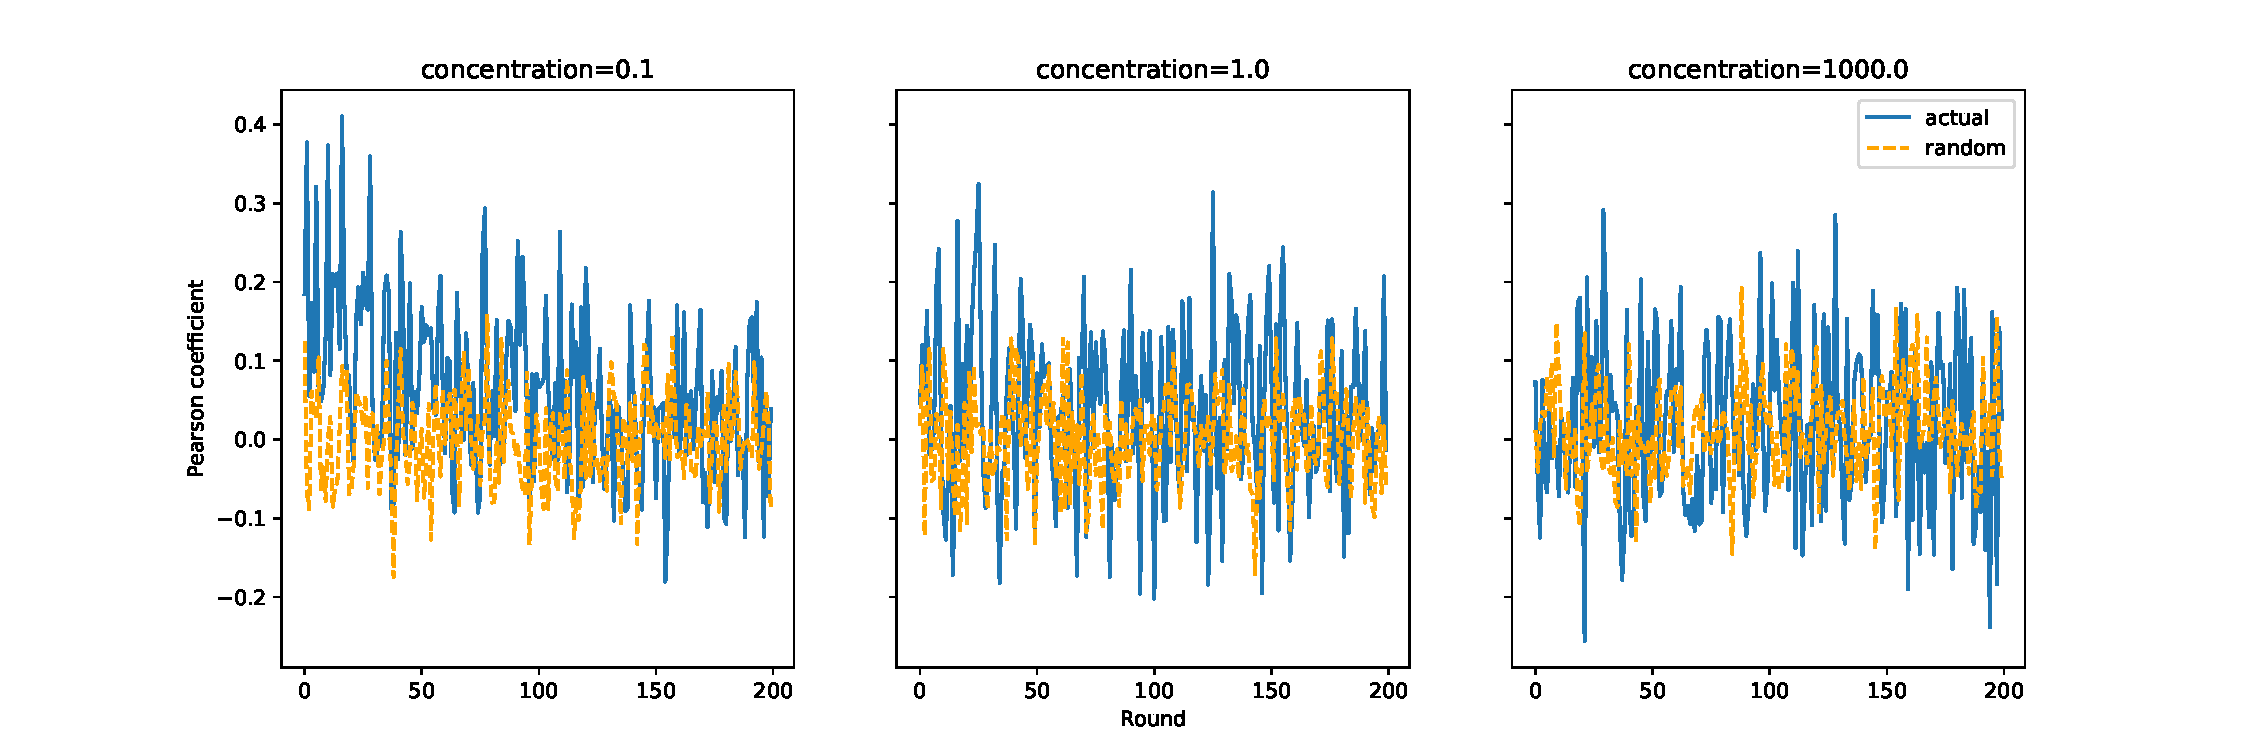
\includegraphics[width=0.8\textwidth]{images/noise_client_pearson_vs_rounds.pdf}
  \caption{Correlation between activation outputs from random noise and client data distribution for each round of training.}
  \label{fig:noise_client}
\end{figure}

\subsection{Centralised Test Activations}
When I instead compare the activations that are given by the centralised test data, I am able to see a stronger correlation, as shown in \cref{fig:test_client}. There is a very noticeable decrease in correlation between the activation outputs of the client models and the client dataset and this decrease is further emphasised after round 150 when the mild exploration phase kicks in and the learning rate decays more drastically. The difference between partitions of different concentrations can also be seen with the partition with concentration of 1000.0 having activation outputs that have almost no correlation at all, most possibly due to the evenly distributed nature of the data.

\begin{figure}
  \centering
  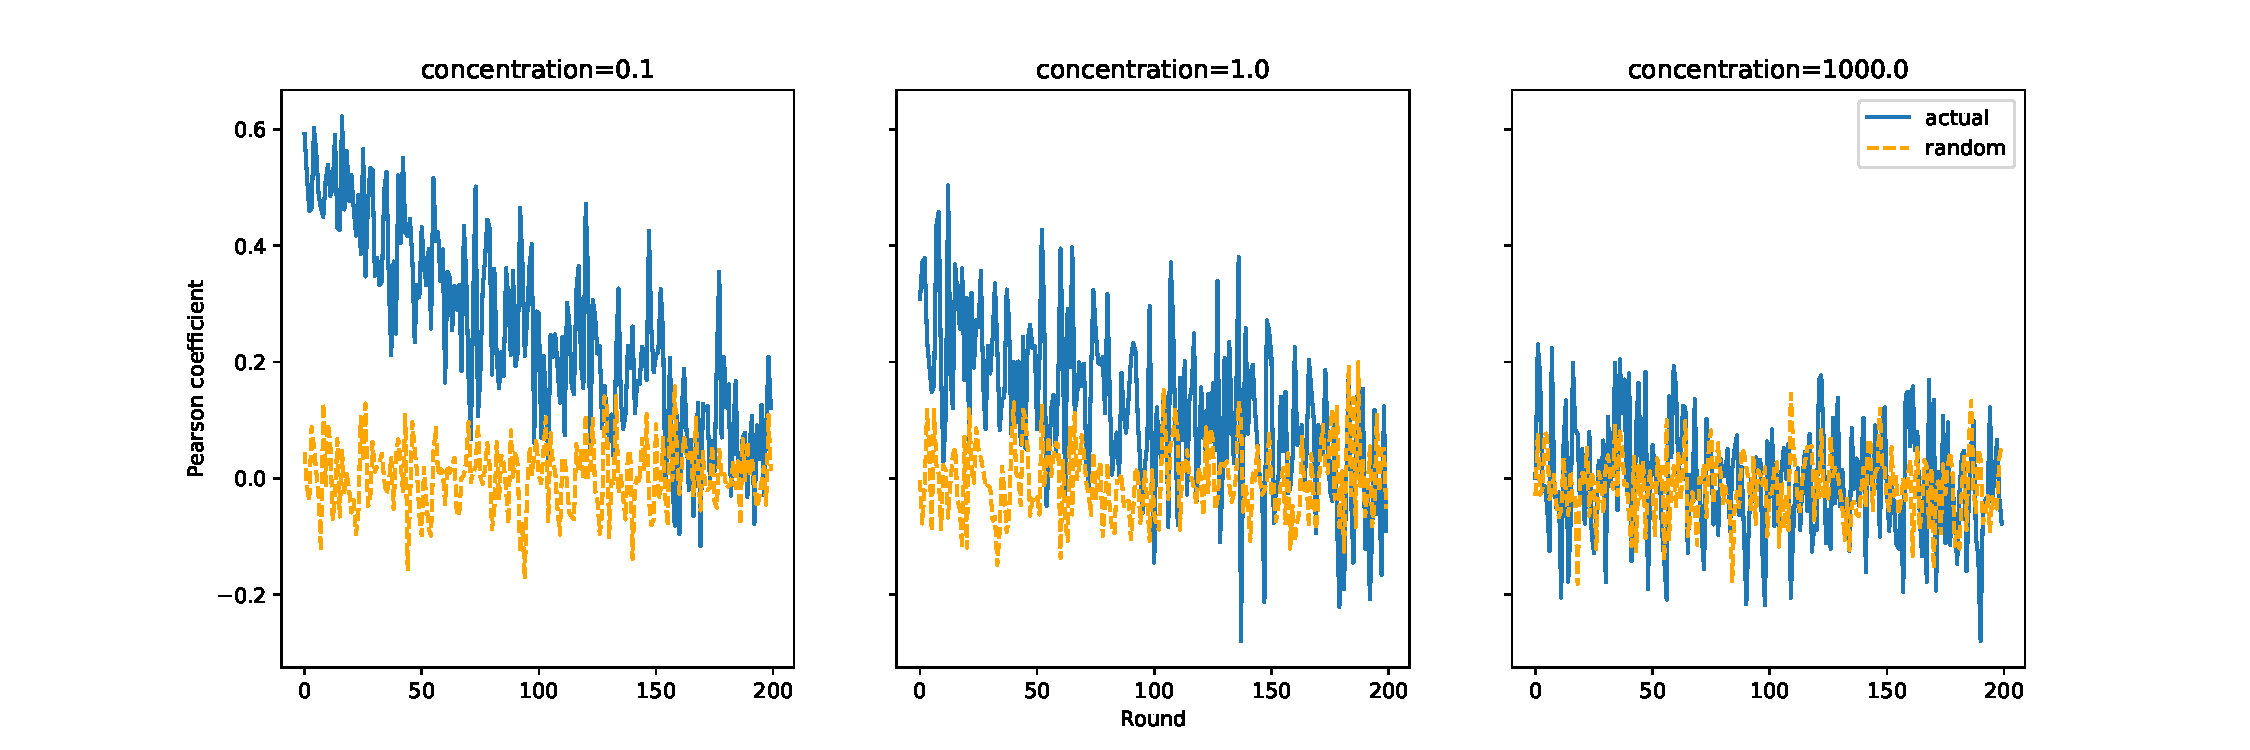
\includegraphics[width=0.8\textwidth]{images/client_pearson_vs_rounds.pdf}
  \caption{Correlation between activation outputs from the client models tested on the centralised test data and client data distribution for each round of training.}
  \label{fig:test_client}
\end{figure}

Changing the approach slightly, I now investigate the change in activation outputs on the centralised test set between the client model and the global model of the previous round. In effect, this isolates the effect of the change to the training on the client alone. The correlations are shown in \cref{fig:change_test_client}. As can be seen, the client models' activations change to fit the data distribution on the client in a highly correlated way. Comparing this to the effects shown in \cref{fig:test_client}, we can say that most likely, the reduction in learning rate and the introduction of IMA prevent these effects from carrying over into the global model.

I check this overall effect by comparing the change in activations of the global model across rounds, as shown in \cref{fig:change_test_global}. To compare this correlation again the data distribution of the 10 clients, I consider a big client whose dataset is the sum of all 10 clients of that round and calculate the correlation between this collated distribution. The results here are less conclusive and highly noisy and I am unable to conclude if this is due to the way in which the activations change when the models are averaged together. Nevertheless, the lack of any significant patterns in the correlations of the global model change despite the strong correlations client models suggest that the effect of \fedavg{} and IMA serve to mitigate the strong stochastic effects of client drift and prevent the model from drifting away from the minimum as well.


\begin{figure}
  \centering
  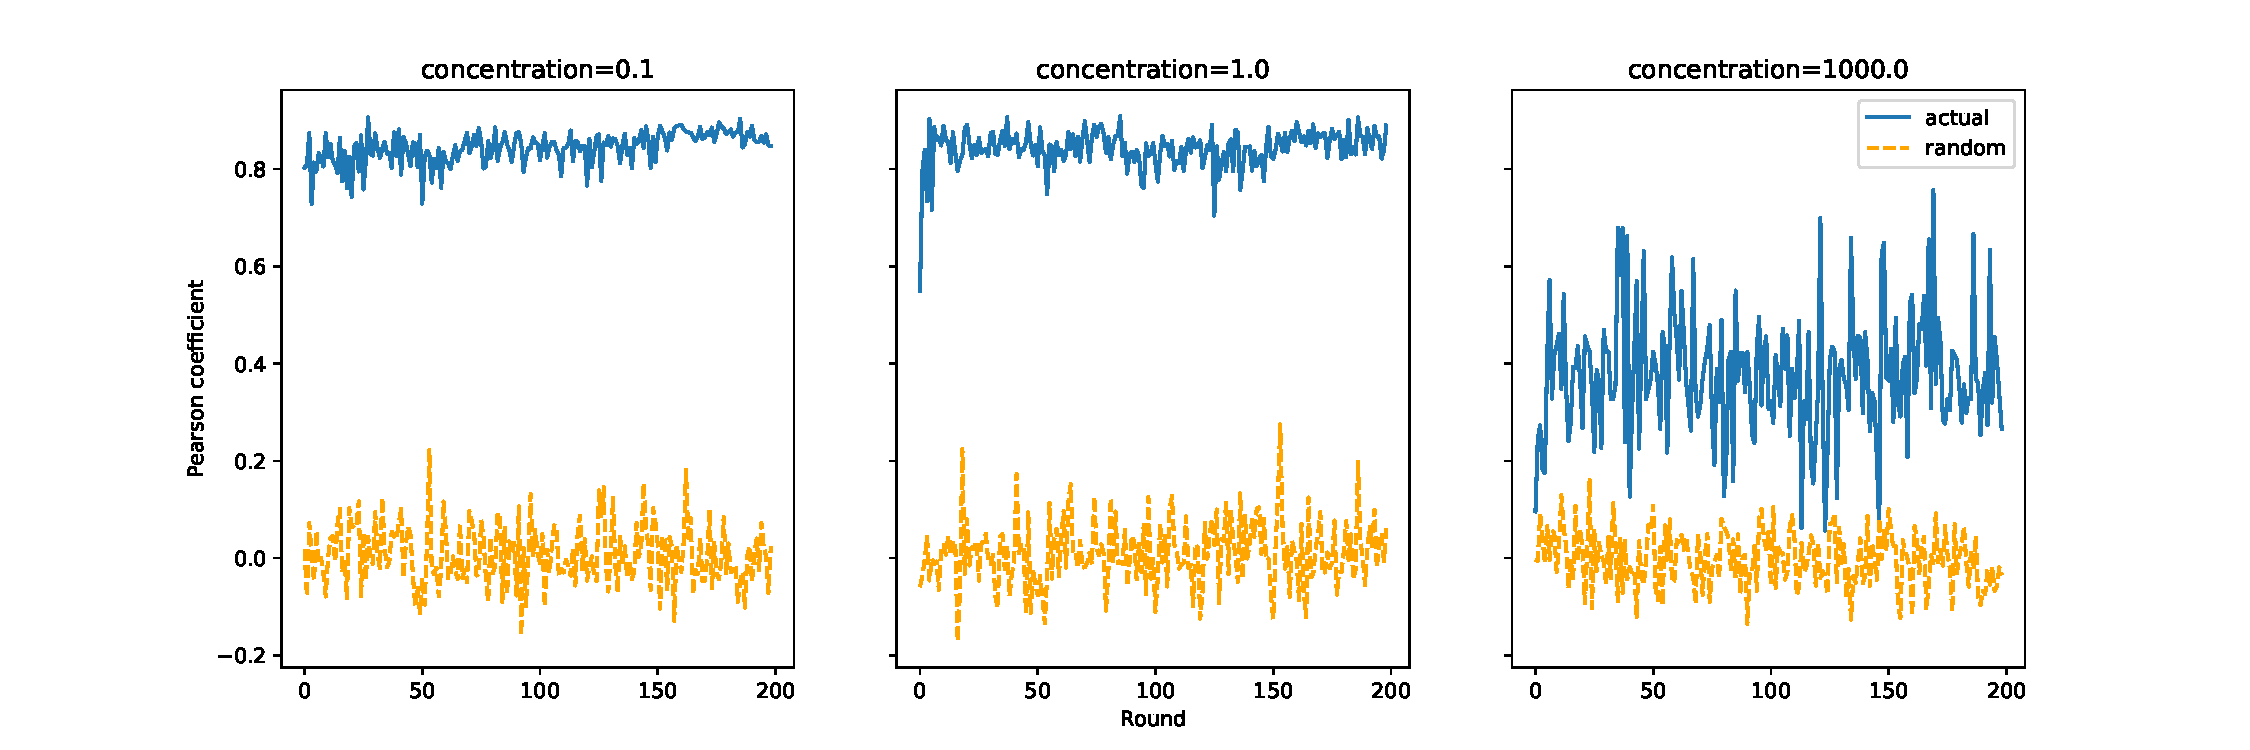
\includegraphics[width=0.8\textwidth]{images/change_prev_client_pearson_vs_rounds.pdf}
  \caption{Correlation between the change in activation outputs from the client models and the previous round's global model tested on the centralised test data and client data distribution for each round of training.}
  \label{fig:change_test_client}
\end{figure}


\begin{figure}
  \centering
  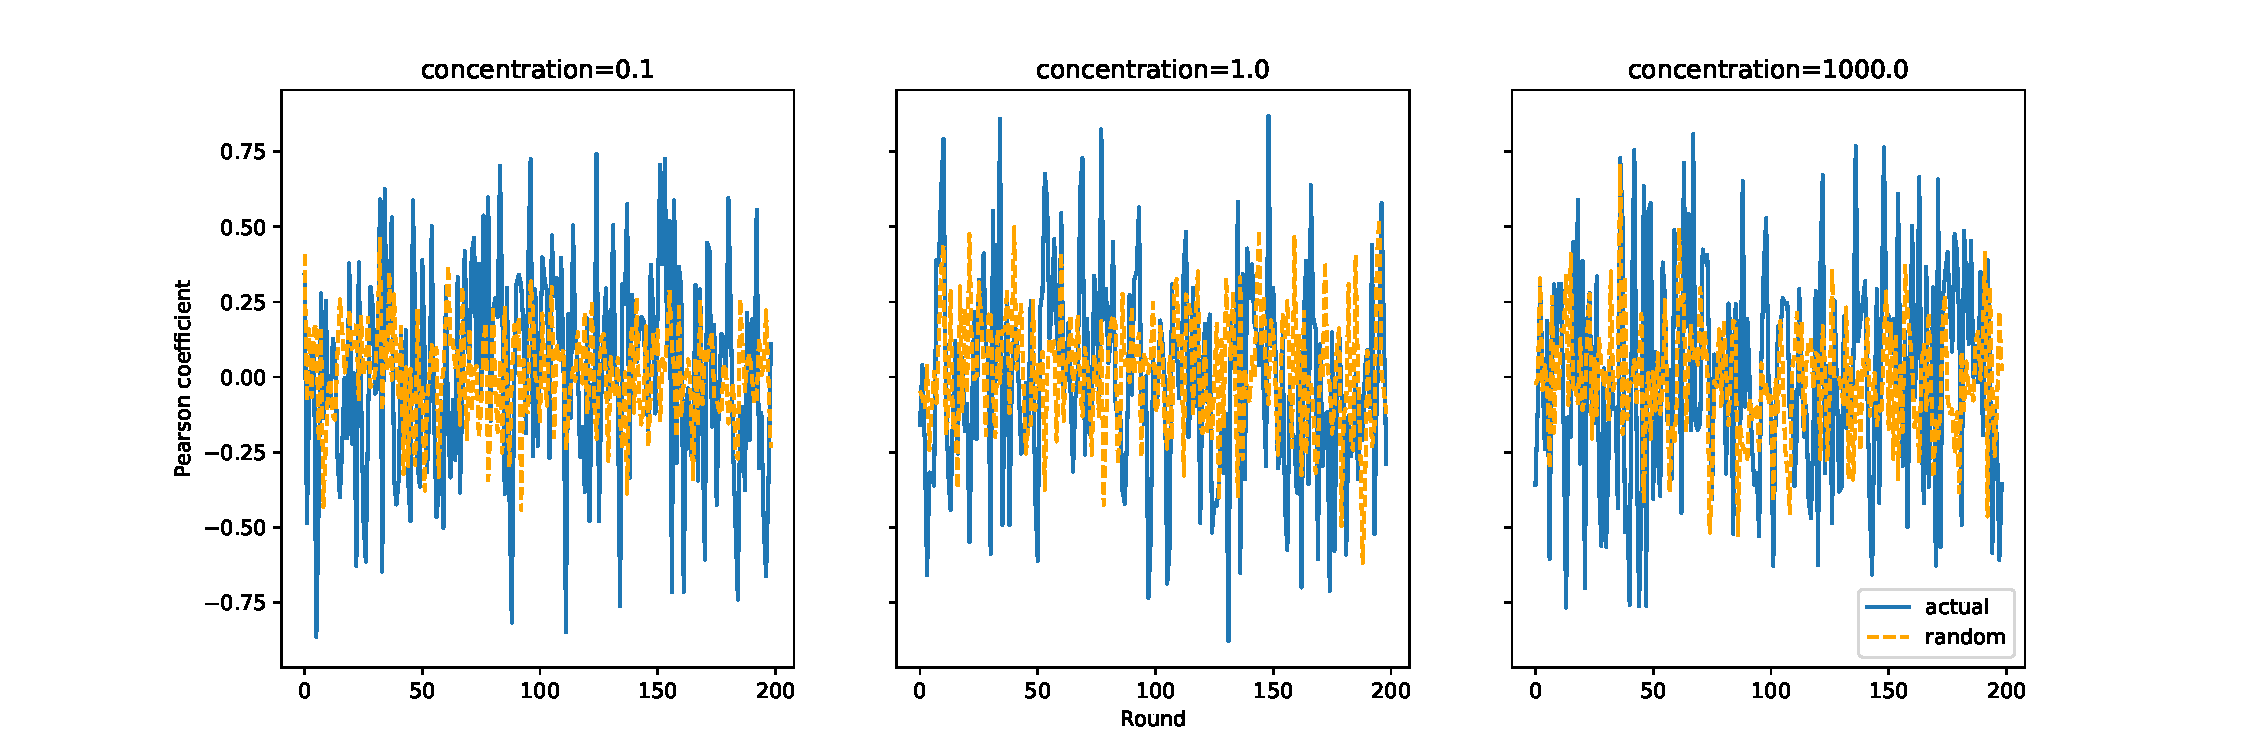
\includegraphics[width=0.8\textwidth]{images/change_prev_global_pearson_vs_rounds.pdf}
  \caption{Correlation between the change in activation outputs between rounds of the global model tested on the centralised test data and client data distribution for each round of training.}
  \label{fig:change_test_global}
\end{figure}

\section{Conclusion}

In conclusion, I show how the model activations are correlated with the label distribution on the client data and how the effect of client drift is very obvious when we look at the activations of the client models. It can be seen how a IMA helps to confine the effects of client drift to the client models and prevents the global model from drifting stochastically with the clients each round.

For further exploration, I think it would be helpful to try IMA without any learning rate decay, or without a mild exploration decay change, so as to isolate the effect of the iterative moving averaging itself. Further study can be done on the confusion matrix as well to see if the precision or recall of each label is correlated with the label distribution in the same way that the activation outputs are.


\bibliographystyle{plainnat}
\bibliography{refs}

%%%%%%%%%%%%%%%%%%%%%%%%%%%%%%%%%%%%%%%%%%%%%%%%%%%%%%%%%%%%
\appendix
\section{Data distribution across all clients}
\label{full-data-dist}
\begin{figure}[h]
  \centering
  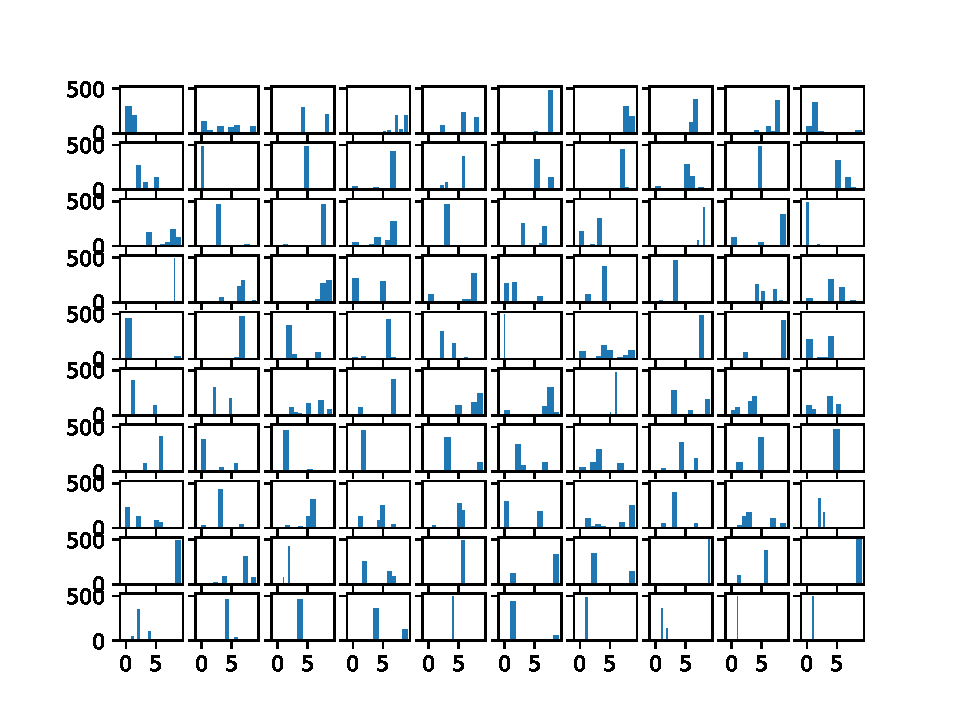
\includegraphics[width=0.9\textwidth]{images/all_data_dist_0.1.pdf}
  \caption{Distribution of labels in all 100 clients with a concentration of 0.1.}
\end{figure}
\begin{figure}[h]
  \centering
  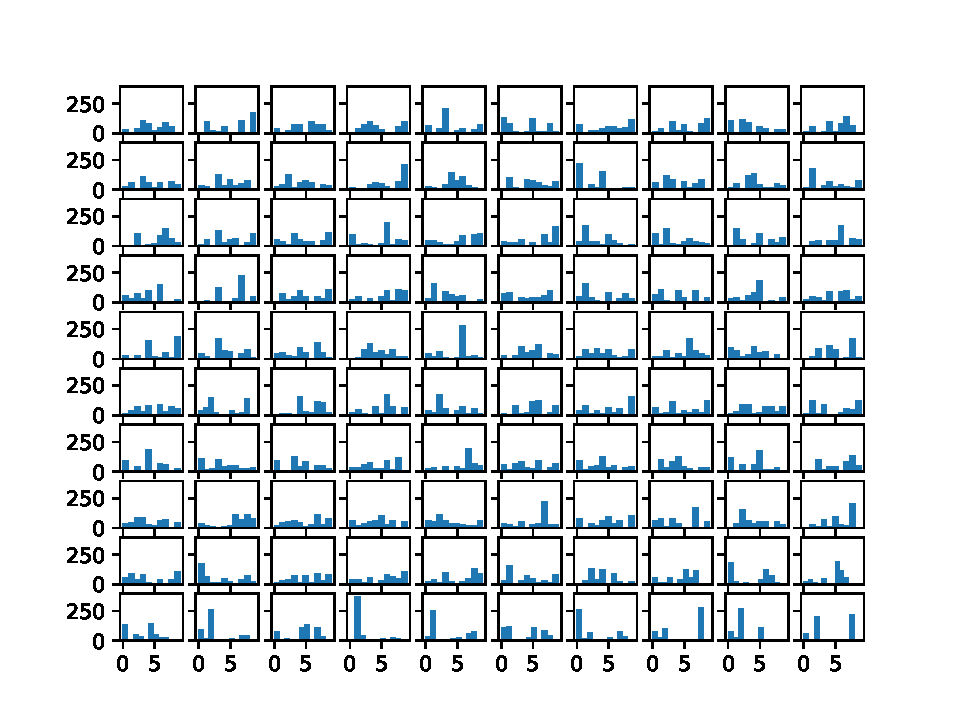
\includegraphics[width=0.9\textwidth]{images/all_data_dist_1.0.pdf}
  \caption{Distribution of labels in all 100 clients with a concentration of 1.0.}
\end{figure}
\begin{figure}[h]
  \centering
  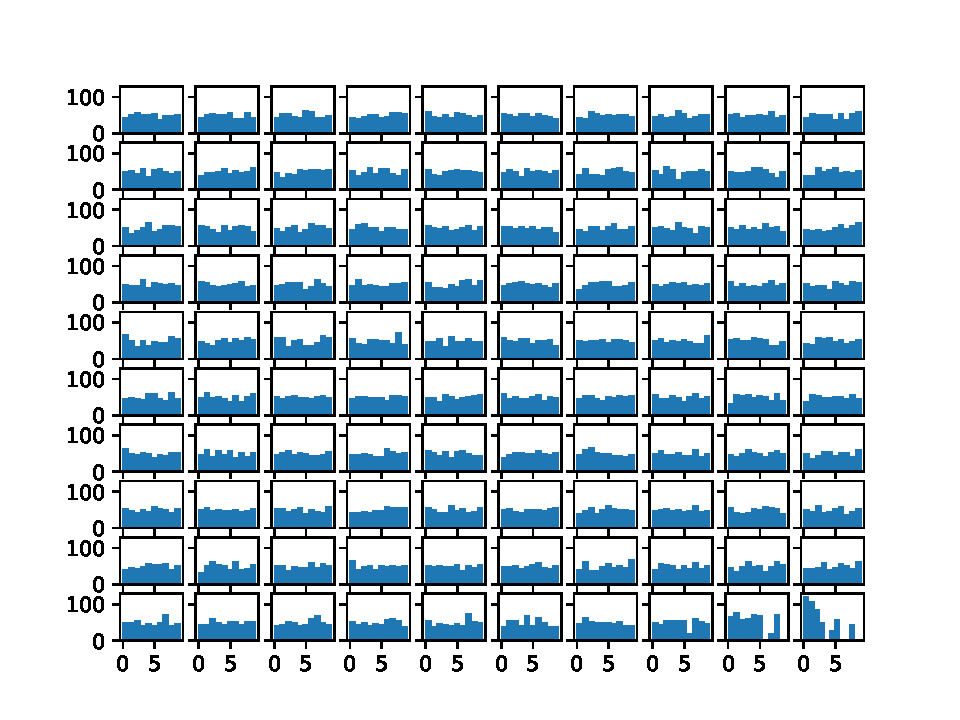
\includegraphics[width=0.9\textwidth]{images/all_data_dist_1000.0.pdf}
  \caption{Distribution of labels in all 100 clients with a concentration of 1000.0.}
\end{figure}

\end{document}